\chapter{Introduction}
\label{chp:chapter1}
\graphicspath{{figures/}{figures/chapter1/}}
\pgfplotsset{
    table/search path={{figures/chapter1/data},{data}},
}

In classical finite element analysis, $80\%$ of overall analysis time is devoted to mesh generation and cleanup, whereas only $20\%$ of overall time is actually devoted to analysis~\cite{cottrell2009isogeometric}. Isogeometric analysis, introduced by Hughes et al.~\cite{HUGHES20054135}, leverages computer aided design (CAD) representations directly in finite element analysis (see Figure~\ref{fig:flow_chart}). It has been shown that this approach can alleviate the model preparation burden of going from a CAD design to an analysis model and improve overall solution accuracy and robustness~\cite{bazilevs2006isogeometric, da2011some, da2014mathematical}. Additionally, the higher-order smoothness inherent in CAD basis functions make it possible to solve higher-order partial differential equations, e.g. the biharmonic equation~\cite{kapl_isogeometric_2015, kapl_isogeometric_2017}, the Kirchhoff-Love shell problem~\cite{kiendl2009isogeometric, kiendl2010bending, kiendl2015isogeometric} and the Cahn-Hilliard equation~\cite{gomez2008isogeometric, borden2014higher} directly without resorting to complex mixed discretization schemes.\par

\begin{figure}[ht]
	\captionsetup[subfigure]{labelformat=empty, font = footnotesize}
	\centering
	\begin{subfigure}[b]{0.47\textwidth}
		\centering
		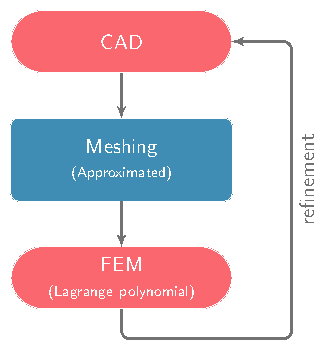
\includegraphics[scale=1.2]{flow-chart-fem}
		\caption{FEA workflow}
	\end{subfigure}
	\begin{subfigure}[b]{0.47\textwidth}
		\centering
		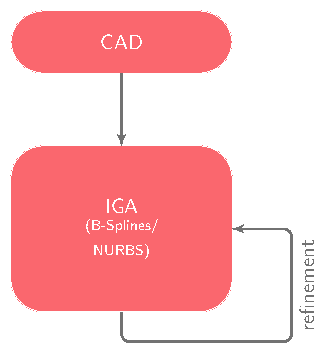
\includegraphics[scale=1.2]{flow-chart-iga}
		\caption{IGA workflow}
	\end{subfigure}
	\caption{A comparison of between classical finite element analysis workflow and isogeometric analysis workflow. FEA workflow: meshing and cleanup are required. Note that the meshing process does not preserve the original CAD geometry. IGA workflow: using the CAD model directly in the finite element analysis. }
	\label{fig:flow_chart}
\end{figure}

CAD models are often built from collections of non-uniform rational B-splines (NURBS). Adjacent NURBS patches often have inconsistent knot layouts, different parameterizations, and may not even be physically connected. Additionally, trimming curves~\cite{kim2009isogeometric, schmidt2012isogeometric} are often employed to further simplify the design process and to extend the range of objects that can be modeled by NURBS at the expense of further complicating the underlying parameterization of the object. While usually not an issue from a design perspective, these inconsistencies in the NURBS patch layout, including trimming, must be accommodated in the isogeometric model to achieve accurate simulation results. As shown in Figure~\ref{fig:geometries}, two primary approaches are often employed. First, the exact trimmed CAD model, shown in Figure~\ref{fig:geometries} in the middle, is used directly in the simulation~\cite{schmidt2012isogeometric}. To accomplish this requires additional algorithms for handling cut cells and the weak imposition of boundary conditions and may result in reduced solution accuracy and robustness. Second, the CAD model is reparameterized~\cite{xu2014high}, as shown in Figure~\ref{fig:geometries} on the right, into a watertight spline representation like multi-patch NURBS, subdivision surfaces~\cite{peters2008subdivision}, or T-splines~\cite{sederberg_t-splines_2003} which can then be used as a basis for analysis directly. The reparameterization process often results in more accurate and robust simulation results but is only semi-automatic using prevailing approaches. In both cases, existing techniques are primarily surface-based due to the predominance of surface-based CAD descriptions.

\begin{figure}[ht]
	\captionsetup[subfigure]{labelformat=empty, font = footnotesize}
	\centering
	\begin{subfigure}[b]{0.32\textwidth}
		\centering
		\includestandalone[scale=.7]{geometry}
		\caption{A geometry}
	\end{subfigure}
	\begin{subfigure}[b]{0.32\textwidth}
		\centering
		\includestandalone[scale=.7]{trimmed_geometry}
		\caption{Trimmed model}
	\end{subfigure}
	\begin{subfigure}[b]{0.32\textwidth}
		\centering
		\includestandalone[scale=.7]{reparameterized_geometry}
		\caption{Reparameterized model}
	\end{subfigure}
	\caption{A geometry and two modelling strategies: trimming and reparameterization.}
	\label{fig:geometries}
\end{figure}

From the analysis perspective, the main challenge for conducting finite element analysis over a geometry consisting of multiple spline patches is how to efficiently and accurately exchange information among different patches. In this dissertation, we focus on the \textit{dual mortar method}, which can robustly apply constraints over intersections of reparameterized multi-patch geometries.  

\section{State of the art}

Researchers in both the design and analysis communities have made significant progress in handling multi-patch NURBS models and the connections between adjacent patches. In this section, we present a brief review of patch coupling techniques developed in both communities. 
\subsection{Local refinable splines}

\begin{figure}[h]
    \centering
    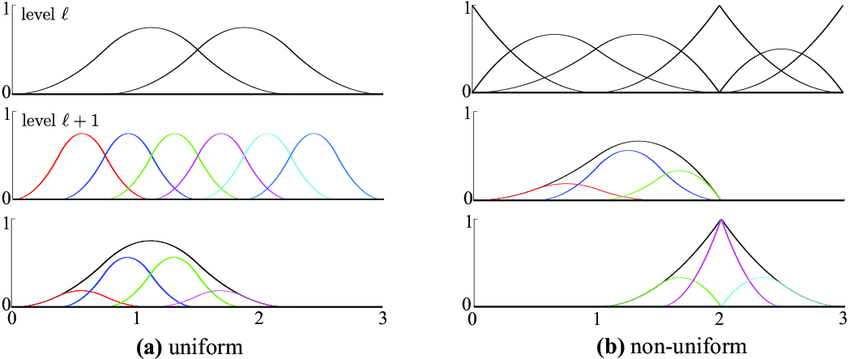
\includegraphics[width=.8\linewidth]{hierarchical-bsplines}
    \caption{Subdivision of B-spline basis functions: (a) Uniform, and (b) non-uniform B-spline basis functions are represented by linear combinations of refined basis functions~\cite{hennig2016bezier}.}\label{fig:hierarchical-bsplines}
\end{figure}

 In order to represent complex topologies, subdivision schemes (Figure.~\ref{fig:hierarchical-bsplines}) are widespread in geometry processing and computer graphics. Subdivision schemes allow for the construction of smooth spline bases over unstructured meshes. Among the most popular subdivision schems are the Catmull-Clark \cite{catmull_recursively_1978}, Doo-Sabin \cite{doo_behaviour_1978} and Loop's \cite{loop_smooth_1987} scheme. For isogeometric analysis, Wei \textit{et al.} \cite{wei_truncated_2015} introduced truncated hierarchical Catmull-Clark subdivion that can handle extraordinary nodes involved in complex topologies. Truncated hierarchical Catmull-Clark subdivion inherits the surface continuity of Catmull-Clark subdivision, namely $C^1$ continuity at extraordinary points and $C^2$ continuity elsewhere. Loop subdivision surfaces provide similar regularity properties as truncated hierarchical Catmull-Clark subdivion and have been applied to isogeometric analysis in \cite{kang_truncated_2016,pan_isogeometric_2015} to generate triangular meshes. One of the limitations in the implementation of subdivision meshes is that the basis function around the extraordinary point is composed of piecewise polynomial functions with an infinite number of segments, which leads to insufficient integration by Gauss quadrature. To deal with this issue, various quadrature rules and adaptive strategies have been examined in \cite{nguyen_comparative_2014} for the Poisson problem on the disk and in \cite{juttler_numerical_2016} for fourth order partial differential equations. \par

\begin{figure}[h]
    \centering
    \begin{subfigure}[b]{0.45\textwidth}
        \centering
        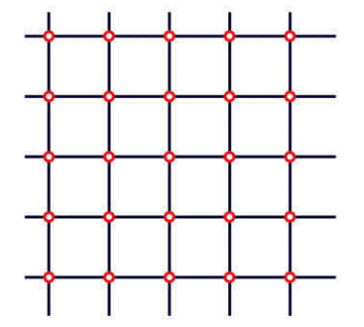
\includegraphics[width=\linewidth]{bspline-control-grid}
        \caption{B-splines}
    \end{subfigure}
    ~
    \begin{subfigure}[b]{0.45\textwidth}
        \centering
        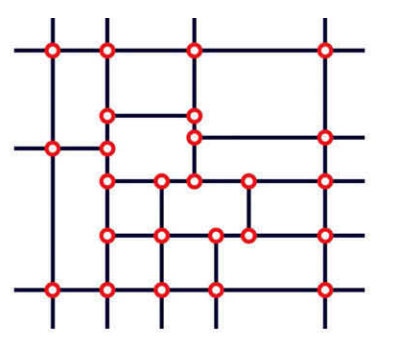
\includegraphics[width=\linewidth]{tspline-control-grid}
        \caption{T-splines}
    \end{subfigure}   
    \caption{Control points lie in a rectangular grid. (a) Topology of B-spline control grid. (b) Topology of T-spline control grid. Note that the presence of T-junction control points is allowed~\cite{bazilevs_isogeometric_2010}.}\label{fig:Tspline-control-grid}
\end{figure}

\begin{figure}[h]
    \centering
    \begin{subfigure}[b]{0.45\textwidth}
        \centering
        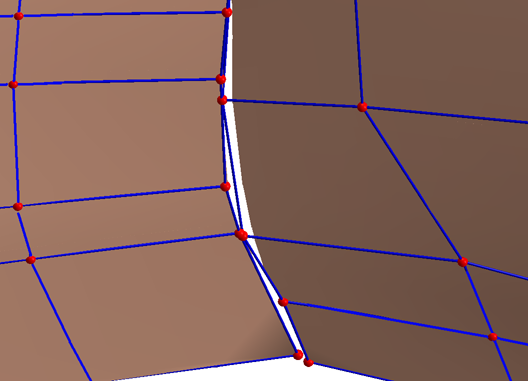
\includegraphics[width=\linewidth]{bspline-two-patch}
        \caption{B-splines}
    \end{subfigure}
    ~
    \begin{subfigure}[b]{0.45\textwidth}
        \centering
        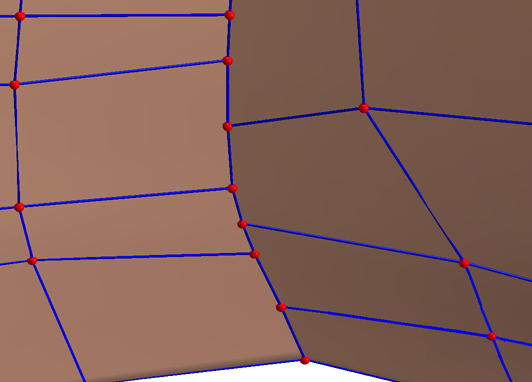
\includegraphics[width=\linewidth]{tspline-two-patch}
        \caption{T-splines}
    \end{subfigure}   
    \caption{A gap between two B-spline surfaces, fixed with a T-spline~\cite{sederberg_t-splines_2003}.}\label{fig:Tspline-two-patch}
\end{figure}

In 2003, Sederberg \textit{et al.} \cite{sederberg_t-splines_2003} introduced T-splines, which allow for the existence of T-junctions in the mesh, so that lines of control points need not traverse the entire mesh. Thus, local refinement can be realized by introducing T-junctions (see Figure.~\ref{fig:Tspline-control-grid}) around interested region. Since the concept of T-splines is a generalization of NURBS technology, it can also be used to merge NURBS surfaces that have different discretizaitons at the intersection (see Figure.~\ref{fig:Tspline-two-patch}). Due to the desirable features of T-splines, Bazilevs \textit{et al.} \cite{bazilevs_isogeometric_2010} explored this technology in isogeometric analysis, and numerical results demonstrated its potential for solving structural and fluid problems. By utilizing the B\'ezier extraction operator, a finite element data structure for T-splines \cite{scott_isogeometric_2011} were developed to ease the incorporation of T-splines into existing finite element codes. However, it has been proven \cite{buffa_linear_2010} that the original definition of T-splines is not sufficient to ensure the linear independence of the basis functions. To circumvent this issue, analysis suitable T-splines \cite{li_linear_2012} were developed by applying an additional constraint that no two orthogonal T-junction extensions are allowed to intersect. Subsequently, the mathematical properties of analysis suitable T-splines were studied in \cite{li_analysis-suitable_2013,xin_li_properties_2015}, and it has been sucessfully applied to the boundary element method \cite{scott2013isogeometric}. Meanwhile, an adaptive local h-refinement algorithm with T-splines and a local refinement of analysis-suitable T-splines were introduced by D\"{o}fel \textit{et al.} \cite{dorfel_adaptive_2010} and Scott \textit{et al.} \cite{scott_local_2012}, respectively. However, for both algorithm, the refined mesh is not as local as one would hope and this problem might be severe in 3D.\par

\subsection{Multi-patch geometrically continuous functions}

One of the advantages of isogeometric analysis is that it provides basis functions with high smoothness, \textit{i.e.} for $p$-th order splines, they enjoy up to $C^{p-1}$ continuity within a single patch. Thus, it is possible to directly discretize differential operators of order higher than 2. However, continuity higher than $C^0$ for multi-patch discretization imposes significant difficulties. The conception of geometric continuity is a well-known and highly useful concept in geometric design \cite{peters_chapter_2002, peters_joining_1992}. The parametric continuity requires both the smoothness of the geometry and its parameterization, whileas the geometric continuity only requires the smoothness of the geometry. Hence, the geometric continuity of order $s$ ($G^s$ continuity) is a weaker continuity constraint as compared to $C^s$ parametric continuity. Bercovier \textit{et al.} \cite{bercovier_smooth_2014} has shown that for multi B\'ezier patches over an unstructured quadrilateral mesh, as long as the order of polynomial is high enough, there always exists the minimal determining set for a $G^1$ continuity construction. Moreover, the resulting basis functions do not contain subdivisions around extraordinary vetices.\par

The case of $G^1$ continuous functions on bilinearly parametrized two-patch B-spline domains was considered by Kapl \textit{et al.} \cite{kapl_isogeometric_2015}, where the $C^1$ basis functions are constructed and analyzed by numerical tests. It is shown that the space dimensionality heavily depends on the parameterization of two bilinear patch, and optimal convergence is observed on the biharmonic problem. However, over-constrained $C^1$ isogeometric spaces that cause sub-optimal convergence are also observed for certain configurations (\textit{e.g.} two-patch non-bilinear parameterizations and $C^{p-1}$ continuity within the patches for $p$-th order spline space). A theoretical analysis of the cause of this so-called $C^1$ locking phenomenon is provided in \cite{collin_analysis-suitable_2016}, where the analysis-suitable $G^1$ geometry parameterization that allows for optimal approximation of $C^1$ isogeometric spaces, is identified and verified by numerical examples. Kapl \textit{et al.} extended the construction of $G^1$ continuous functions to bilinearly parameterized multi-patch domains in \cite{kapl_isogeometric_2017}, where the simple explicit formulas for spline coefficients of $C^1$ basis function are derived and nested $C^1$ isogeometric spaces are generated. Recently, Kapl \textit{et al.} \cite{kapl_space_2017,kapl_space_nodate} explored the construction of $C^2$ isogeometric functions on multi-patch geometries and utilized the $C^2$ isogeometric spaces for $6$-th order PDE.\par

Although the geometrically continuous functions circumvent the use of subdivisions for domains with extraordinary vertices, the requirement of $C^0$ parameterization averts local mesh refinement, and lower continuity is required to avoid $C^1$ locking effect. Thus, its implementation can be complex and it may not be a potential candidate for analysis in more general situations.\par

\subsection{Variational approaches}

From the analysis perspective, the pointwise satisfaction of continuity constraints between adjacent patches is often unnecessarily rigorous. A reasonable approximation can be achieved even if these constraints are applied in a variational setting. The Lagrange multiplier method is a general framework which can be used to apply constraints to variational problems. In the context of isogeometric analysis, various types of Lagrange multiplier approaches have been applied to problems in solids~\cite{hesch_isogeometric_2012, seitz2016isogeometric} and fluids~\cite{bazilevs2012isogeometric}. While general in applicability, the solvability and optimality of the Lagrange multiplier method is significantly influenced by the \textit{inf-sup} condition~\cite{babuvska1973finite,boffi_mixed_2013}. In the context of domain coupling, to satisfy the \textit{inf-sup} condition, special modifications are needed when building the Lagrange multiplier space to ensure stability (see Figure~\ref{fig:mortar_basis}). This has been further studied in~\cite{bernardi_basics_2005, bernardi_domain_1993, belgacem_mortar_1998, barbosa1991finite} for finite element analysis and in~\cite{brivadis_isogeometric_2015} for isogeometric analysis. \par

Whereas the Lagrange multiplier method applies continuity constraint by Lagrange multipier, leading to a saddle point problem, the mortar method, first introduced by Bernardi~\cite{bernardi_domain_1993}, considers a constrained solution space and gives rise to a positive definite variational problem. Wohlmuth~\cite{wohlmuth2000mortar} used dual basis functions to discretize the Lagrange multiplier spaces, which further simplifies the mortar formulation. Dual basis functions for the piecewise linear elements are illustrated in Figure~\ref{fig:mortar_basis}. A dual mortar method for isogeometric analysis was first developed by Seitz et al.~\cite{seitz_isogeometric_2016}. \par

Applying constraints by the Lagrange multiplier method leads to a saddle point problem, of which the discrete Lagrange multiplier basis functions cannot be chosen independently of that of the primal variable and special treatment is required to ensure the solvability and optimality of the discretized system. The stiffness matrix for the discrete problem arising from the Lagrangian multiplier method always contains both positive and negative eigenvalues, for which iterative methods are known to be less efficient than for symmetric positive definite systems. The perturbed Lagrangian method alleviates these issues by appending a weighted quadratic penalty term to the energy functional. The main drawback of the perturbed Lagrangian method is the inconsistency with the original problem. It has been utilized in \cite{simo1985perturbed} for contact problems and \cite{dornisch2011boundary, apostolatos2015domain} for domain decomposition problems in the isogeometric analysis framework.\par

To fully circumvent the inf-sup condition for imposing Dirichlet boundary conditions by Lagrange multiplier, Barbosa et. al. \cite{barbosa1991finite} added a new penalty like term to the energy functional to enhance the stability. Unlike perturbed Lagrangian methods where the penalty term is inconsistent with the original problem, the new term proposed by Barbosa maintains the consistency. It has been demonstrated that there is a close connection with the stablized Lagrange multiplier method and Nitsche's method in the context of setting the Dirichlet boundary conditions \cite{stenberg1995some} and in the context of domain decomposition \cite{hansbo2005lagrange, hansbo_nitsches_2005, juntunen2015connection}. Tur et. al. \cite{tur2015modified} utilized this method to solve both small and large deformation contact problems and obtained optimal convergence rates for linear elements. To our knowledge, this method has not been applied in the isogeometric analysis framework yet. \par

The discontinuous Galerkin method (or Nitsche's method) was introduced in 1971 \cite{nitsche_uber_1971} for handling Dirichlet boundary conditions in the weak sense. The discontinuous Galerkin method resembles a mesh-dependent penalty method. Unlike the standard penalty method, which is not consistent unless the penalty coefficient goes to infinity, the discontinuous Galerkin method is consistent with the original problem. Moreover, no additional unknown (Lagrange multiplier) is needed and no discrete inf-sup condition must be fulfilled, contrarily to mixed methods. Meanwhile, additional terms are added into the weak form to ensure the ellipticity of the problem. The discontinuous Galerkin method has been widely studied in various aspects, including imposing boundary conditions \cite{hansbo_nitsches_2005}, domain decomposition \cite{becker_finite_2003} and contact problems \cite{chouly_symmetric_2015}. In the field of the isogeometric analysis, the discontinuous Galerkin method has been utilized to impose Dirichlet boundary conditions for trimmed spline meshes \cite{embar_imposing_2010}. The first article discussing the discontinuous Galerkin method based domain decomposition strategy was written by Apostolatos \textit{et al.} \cite{apostolatos_nitsche-type_2014}. Nguyen \textit{et al.} extended it to three-dimensional problems in \cite{nguyen_nitsches_2014}. Guo \textit{et al.} \cite{guo_nitsches_2015} proposed a Nitsche's method for coupling Kirchhoff-Love NURBS shell patches.\par

\begin{figure}
  \centering
  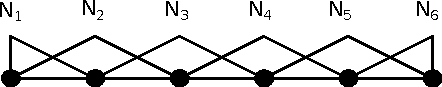
\includegraphics[width=.7\linewidth]{original_basis}\\
  \vspace{1em}
  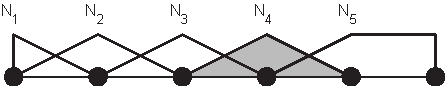
\includegraphics[width=.7\linewidth]{mortar_basis}\\
  \vspace{1em}
  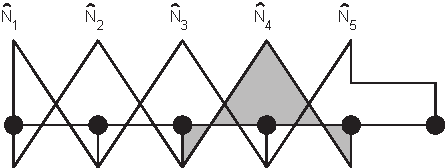
\includegraphics[width=.7\linewidth]{dual_mortar_basis}
  \caption{Lagrange multiplier basis functions for the piecewise linear elements, top: original piecewise linear basis, middle: piecewise linear basis with modification at the right end, bottom: dual basis functions for the piecewise linear elements, modification at the right end (Courtesy of Zienkiewicz~\cite{zienkiewicz1977finite}).}\label{fig:mortar_basis}
\end{figure}

\section{Research contributions}

In this dissertation, the dual mortar framework for most prevailing higher-order partial differential equations (including biharmonic problems, Cahn-Hilliard problems and Kirchhoff-Love shell problems) are developed. The primary contributions of this dissertation are:
\begin{itemize}
    \item Formulation and implementation of an isogeometric B\'ezier dual mortar method for the biharmonic problem on multi-patch domains. The formulation leads to an efficient construction of a sparse constrained linear system. We prove the well-posedness of the formulation and specify requirements to achieve optimal convergence. 
    \item Development of the enriched \Bezier dual basis. The enriched \Bezier dual basis functions are constructed via a quadrature-free algorithm and can reproduce polynomials up to a given degree. 
    \item Formulation and implementation of an isogeometric \Bezier dual mortar method for the Kirchhoff-Love shell problem on multi-patch domains. 
    \item Extension of \Bezier dual basis functions to alleviate transverse shear locking in Timoshenko beams and volumetric locking in nearly compressible linear elasticity. Based on the different interpretation of the $\bar{B}$ formulation, we develop two formulations for locking problems.
    \item An isogeometric analysis code in C++ is developed. Eigen library~\cite{eigenweb} is adopted as the primary linear solver. The assembly routine is multi-threaded by the thread module in the Standard Template Library (STL). This code is capable of handling nonlinear dyanmic problems with higher mesh resolution. 
\end{itemize}

\section{Organization of the dissertation}

The remainder of this thesis is structured as follows: Chapter~\ref{chp:chapter2} provides an overview of isogeometric analysis, e.g. the formulation of B-splines and NURBS, knot insertion and degree elevation algorithms. In addition, the concepts of \Bezier extraction/projection and dual basis functions are explained. In Chapter~\ref{chp:chapter3} the \Bezier dual mortar method for the biharmonic problem is theoretically and numerically studied. The optimality of the proposed formulation requires the \textit{inf-sup} stable as well as a suitable approximation property for the Lagrange multiplier space. However, numerical studies indicate that \Bezier dual basis fails to provide adequate approximation, leading to sub-optimal convergence results. In Chapter~\ref{chp:chapter4}, we investigate all factors that influence the approximation of basis functions and develop the enriched \Bezier dual basis. The enriched \Bezier dual basis, constructed via a quadrature-free algorithm, possesses the polynomial reproduction ability and compact support. The accuracy and robustness of the enriched \Bezier dual basis is thoroughly tested by various $2^\text{nd}$ and $4^\text{th}$ order problems. In Chapter~\ref{chp:chapter5}, the \Bezier dual mortar method for the Kirchhoff-Love shell problem is presented. The formulation is based on a dual mortar compatible constraint and handles both smooth shell coupling problem as well as kinked shell coupling problem. The enriched \Bezier dual basis is adopted as discretized Lagrange multipliers, leading to a sparse linear system. Several linear and nonlinear benchmark problems verify the accuracy and robustness of this approach. In Chapter~\ref{chp:chapter6}, the application of \Bezier dual basis is extended to alleviate transverse shear locking in Timoshenko beams and volumetric locking in nearly compressible linear elasticity without populating the stiffness matrix. Finally, conclusions and directions for future work are given in Chapter~\ref{chp:chapter7}.